%\documentclass[fleqn]{article}
\documentclass{article}
\title{Collapsing Heterogeneous Towers of Interpreters}
\author{Michael Buch}
\date{\today}

\usepackage[inline]{enumitem} % inline numbered lists
\usepackage[left=2cm,right=2cm]{geometry}
\usepackage{verbatim} % for comments
\usepackage{graphicx}
\usepackage{amsmath}
\usepackage{amssymb}
\usepackage[tdiagram]{semantic}
\usepackage{amsthm}
\usepackage{textcomp}
\usepackage{txfonts}
%\usepackage{tikz}
%\usetikzlibrary{matrix}
\usepackage{booktabs}
\usepackage{makecell} % For table formatting
\usepackage{multirow} % For table formatting
\renewcommand\theadfont{\bfseries}

\theoremstyle{definition}
\newtheorem{definition}{Definition}[section]
\newcommand{\ts}{\textquotesingle}

\newcommand{\mslang}{$\lambda_{\uparrow\downarrow}$}
\newcommand{\mslangStar}{$\lambda_{\uparrow\downarrow}^*$}
\newcommand{\mevl}{$M_{e}$}
\newcommand{\secdlisp}{SecdLisp}

\usepackage{stmaryrd}
\usepackage{hyperref}
\hypersetup{
    colorlinks=true,
    linkcolor=blue,
    filecolor=magenta,
    urlcolor=cyan,
}
\urlstyle{same}

% Code style:
\usepackage{minted}
%\RecustomVerbatimEnvironment{Verbatim}{BVerbatim}{} % For centering markup
%\renewcommand{\figurename}{Listing}
\usemintedstyle{vs}

% For Word Count:
\newcommand{\detailtexcount}[1]{%
  \immediate\write18{texcount -merge -sum -q #1.tex lit_review.bbl > #1.wcdetail }%
  \verbatiminput{#1.wcdetail}%
}
 
\newcommand{\quickwordcount}[1]{%
  \immediate\write18{texcount -1 -sum -merge -q #1.tex lit_review.bbl > #1-words.sum }%
  \input{#1-words.sum} words%
}
 
\newcommand{\quickcharcount}[1]{%
  \immediate\write18{texcount -1 -sum -merge -char -q #1.tex lit_review.bbl > #1-chars.sum }%
  \input{#1-chars.sum} characters (not including spaces)%
}

\begin{document}
\maketitle
\frenchspacing

%%TC:ignore
%\quickwordcount{lit_review} (out of 15000)
%\quickcharcount{lit_review}
%\detailtexcount{lit_review}
%%TC:endignore

\tableofcontents

\begin{abstract}
Intuitively towers of interpreters are a program architecture by which sequences of interpreters interpret each other and a user program is evaluated at the end of this chain. While one can imagine such
construct in everyday applications, prior research made use of towers of interpreters as a foundation to model reflection. As such, towers of interpreters in literature are synonymous with reflective towers and provide a tractable method with which to reason about reflection and design reflective languages. As a result, the assumptions and constraints that govern tower models make them unapplicable to practical or non-functional
settings. Prior formalizations of reflective towers have identified partial evaluation and reflection to harmonize in the development of such towers. We lift several restrictions of reflective towers including reflectivity, meta-circularity and homogeneity of data representation and then construct non-reflective towers
of interpreters to explore how partial evaluation techniques can be used to effectively remove levels of interpretation within such systems. %We then extend formalisms to such setting and go on to generalize previous techniques on partially evaluating towers of interpreters.
\end{abstract}

%TODO redraw tombstone diagarm using semantic pkg
%\begin{picture}(220,75)(0,-35)
%\put(10,0){\interpreter{S,L’}}
%\put(110,0){\program{P,\compiler{C,\machine{M},\program{P,M}}}}
%\end{picture}

\section{Introduction}
Towers of interpreters are a program architecture which consists of sequences of interpreters where each interpreter is interpreted by an adjacent interpreter in the tower. On one hand, it has been used in the formalization of reflection in LISP and serves as a model in the development of reflective languages. On the other hand, towers of interpreters are a frequent occurrence in application development. Examples include interpreters for embedded domain-specific languages (DSLs) or string parsers embedded in a language both of which form towers of two levels. Advances in virtualization technology has driven increasing interest in software emulation. Viewing emulation as a form of interpretation we can view interpreters running on virtual hardware as towers of interpreters as well.

The inefficiency of reflective tower models of evaluation has been noted since their inception.
CAN COMPILE REFLECTIVE LANGUAGES
REMOVE LAYERS OF INTERPRETATION
COMPILING WITH MODIFIED COMPILED SEMANTICS

% TODO: interpreters should be evaluators
%TODO: stronger first sentence that summarizes contributions, non-metacircular -> heterogeneous
In our study we investigate previous work on collapsing towers of interpreters and aim to take another step towards applying these techniques to real-world settings. We demonstrate that given a multi-level language and a lift operator we can stage individual interpreters in a sequence of non-metacircular interpreters and effectively generate code specialized for a given program eliminating interpretative overhead in the process. As part of the development of this framework our contributions include:
\begin{enumerate*}[label=(\arabic*)]
	\item the development of extensions to the SECD machine that allow it to be staged
	\item implementation of a compiler from a minimal LISP-style language to instructions of the staged SECD machine
	\item demonstration of collapsing towers of interpreters built on top of the aforementioned SECD machine
	\item evaluate the effect of staging at different interpreters within a tower of interpreters
	\item demonstrate the ability to use NbE-style lift operators to perform partial evaluation across levels in the tower that are compilers
	\item and finally evaluation of the structure of the generated code and possible optimizations
\end{enumerate*}.

%We deviate from traditional research in reflective towers in that we do not develop a separate language that demonstrates reflective tower capabilities and part from the constraints of metacircularity and reflection.
%Instead of generating levels in the tower dynamically through reflection and reification operators we construct a pre-determined tower resembling towers of interpreters in practice. We demonstrate initially how meta-circularity and reflection eases the collapsing process and then wire the tower in a way that breaks key implicit assumptions of said technique. Finally we propose a generalization of the original framework that deals with the constraints such a semantic gaps and lack of reflection and reification. We evaluate the framework on a set of abstract machines that are convenient to implement in Lisp-like fashion but are capable of modelling a broad set of functional and non-functional language properties.

One of the aims of this study is to explore the effectiveness of compilation of towers under various configurations. The expected outcome follows the Amin et al.'s idea of only staging the user-most interpreters for the most efficient code output.
effect of staging at different levels
how severe is the difference in generated code? is it worth the increased implementation complexity?

\cite{jones1993partial}: page 26. Only recently has partial evaluation seen growing adoption with frameworks such as Scala's LMS \cite{rompf2010lightweight} or Oracle's GraalVM \cite{wurthinger2013one}. The design space of partial evaluators is multi-faceted and considerations include:
\begin{itemize}
	\item use of mixed languages (Futamura's mix for compilation requires same PE input language as mix is written in)
	\item accept different types of interpreters with different semantics (this is what we partly address) (and what GraalVM addresses?)
	\item performance
	\item BTA strategy: automatic or manual? offline or online? how to deal with non-termination?
	\item Heuristics for guiding PE to produce efficient/desirable code (e.g. you cannot say of a compiler that it doesn't produce more valuable program transformation. But PE's accept that some applications do not warrant it. How to detect such situations?)
\end{itemize}

semantic gap has been discussed previously as a challenge outstanding in the study of partial evaluation.

Chapter 17: specifcies partial evaluation in the context of general program transformation and outlines PE research areas

TODO:
staging vs pe
partial evaluatability of SECD (and other linear interpreters/small step semantics vs denotational/big step/recursive descent parsers)
retaining info in PE of TDPE style (our strategy is thunks)
contribution: was natural to start with EBASE but uncovered problems BLANK
tying the knot in the code instead of data
transfer whiteboard diagram
are able to stage/lift through compiler/translator
structurally similar/equal to javascript tower
implementations:
	1. regular expression matcher (on metaeval or in place of metaeval)
	2. try/catch
	3. using cps adding amb (needs set! and store => turn metaeval into cesk machine (possible because SECD supports recursion, lambdas, letrec, etc.))
Our collapsing strategy is based on the fact that we can choose to either evaluate code or generate code which is an inherent property of the multi-level language base \mslang. Thus in a realistic tower base needs to be a multi-level language

Partial evaluators can be thought of as lightweight optimizing compilers targeting specific optimization goals

% https://tex.stackexchange.com/questions/181366/drawing-tombstone-diagrams
% https://proglang.informatik.uni-freiburg.de/teaching/compilerbau/2004/T-diagrams.pdf
% TODO: use http://mirror.its.dal.ca/ctan/macros/latex/contrib/semantic/semantic.pdf package to draw diagram
% TODO: draw diagram for practical tower as well
\begin{figure}[t]
	\centering
	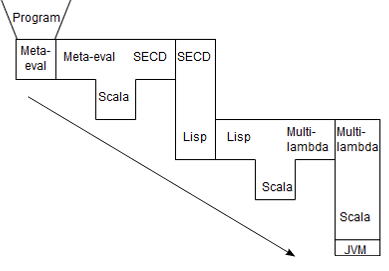
\includegraphics[scale=2]{tombstone_tower.png}
	\label{fig:tombstone}
	\caption{A tombstone digram representation of our framework}
\end{figure}

The aim of our study is to explore the process of turning towers of interpreters into compilers by staging appropriate interpreters and provide a launching point for further research into the optimization of mixed-language systems using partial evaluation.

In section \ref{sec:background} we explain potentially useful background information that cover the fundamental topics we base our framework and experiments starting from the link between interpreters and compilers up to how previous work compiled reflective towers. Section \ref{sec:mslang} provides an overview of the partial evaluation framework we base our study on called Pink \cite{amin2017collapsing}. We systematically describe the process by which we create a heteregeneous tower of interpreters and incrementally collapse in sections \ref{sec:secd} through \ref{sec:collapsing}. Each of these sections discusses the steps we took to create a level in the tower of interpreters as shown in figure \ref{fig:tombstone}. We conclude with an evaluation of experimental results followed by a discussion of potential future work in sections \ref{sec:conclusion} and \ref{sec:future} respectively.

\section{Background}\label{sec:background}
\subsection{What are Interpreters?}
Interpreters vs. compilers
Lines are getting blurry: JIT compilation or more recently Graal
But the Futamura showed they are fundamentally related in an elegant way by three projections that follow from the SMN theorem in recursive function theory
What follows is the study of partial evaluation which lies at the heart of our methodology of collapsing towers of interpreters and is described in more detail in SECTION

\subsection{Type-Directed Partial Evluation (TDPE)}
NbE resources:
%Useful \href{http://cs.ioc.ee/ewscs/2009/dybjer/mainPalmse-revised.pdf}{Slides}
%\href{http://www.cse.chalmers.se/~abela/univnbe.pdf}{NBE paper}
%\href{http://homepages.inf.ed.ac.uk/slindley/nbe/nbe-cambridge2016.pdf}{More slides}
%\href{https://www.microsoft.com/en-us/research/wp-content/uploads/2016/07/supercomp-by-eval.pdf?from=http%3A%2F%2Fresearch.microsoft.com%2Fen-us%2Fum%2Fpeople%2Fsimonpj%2Fpapers%2Fsupercompilation%2Fsupercomp-by-eval.pdf}{Supercompilation by Evaluation}
%\href{http://citeseerx.ist.psu.edu/viewdoc/download?doi=10.1.1.630.2123&rep=rep1&type=pdf}{Supercompilation and Normalization by Evaluation}

Alternative techniques include syntax directed partial evaluation and off-line partial evaluation
Futamura's second project showed the direct relationship between an interpreter and a compiler -> hard to realize
Jone's et al. developed MIX which was the first self-applicable PE that operated on a language developed by the same authors called MIXWELL.
MIX innovated by making binding-time decisions offline as opposed to during partial evaluation time using source annotations for the PE
However as noted in \cite{grobauer2001second}, traditionally partial evaluation worked on untyped languages where a single universal datatype could represent all static values
PE of typed languages was one of the challenges with PE outlined by Jones \cite{jones1988challenging}.

Differences to traditional syntax-directed offline partial evaluators (like MIX):
* binding time is automatic (or requires annotations only on inputs to program e.g. like in Pink, which requires knowledege of how the binding-time works. TDPE only requires annotations on base types from which product, sum and function types' binding-times can be deduced. Pink does not necessarily have a binding time analysis step which makes it slightly more convenient for manual annotation)
* type-directed means we use the type of a term to guide the normalization (i.e. ``extraction function'' is parameterized by type)
* TDPE reuses underlying evaluator to perform static evaluation vs code generation. Traditionally these are performed by the partial evaluator separately in the form of symbolic computation on the source. Pink takes the former approach

In \cite{danvy1999type} Danvy builts a language in ML that supports and reflection (section 1) and then shows how partial evaluation of can be achieved using a ``normalization function'':
%In  summary,  if  one  implements  the  two-level  lambda-calculus  as  in  Sec-tion  1.3, then reifying  a simply typed,  closed, and completely static  higher-order  function  into  a  dynamic  expression  automatically  yields  a  representation  of  its  normal form.  In the rest  of this section,  we illustrate this phenomenon  with  de-compilation,  before  turning to the  implementation  of  a normalization  function  in  ML.

page 379 explains role of let-insertion
Our framework uses the Eijiro Sumii  approach

page 388: actual description of TDPE
"We  define  type-directed  partial  evaluation  as normalization  by  evaluation  over  ML values"

page 403: benefits of NbE

\cite{jones1993partial} page 103: monovariance, polyvariance, congruence in PE

\subsection{Staging}
There are two types of partial evaluation methodologies \cite{jones1993partial}:
\begin{itemize}
	\item Offline partial evaluation
	\item Online partial evaluation \cite{cook2011tutorial}
\end{itemize}
Namin et al. \cite{amin2017collapsing}, propose two languages Pink and Purple. Pink uses a form of online partial evaluation (driven by whether values are "code?" or not) but requires manual staging facilities. Purple relies on LMS for automatic binding time analysis and staging
which limits it to offline partial evaluation and thus relies on further optimization heuristics to achieve the same level of program specialization in the generated code as Pink.
at its heart it uses the fact that $\beta$-reduction to $\beta$-normal form can be viewed as a form of specialization (taken further by NbE \cite{berger1991inverse,berger1998normalization})
``NbE'' extracts the normal form from its meaning (i.e. semantics -> syntax or in our case Val -> Exp which is done via the ``lift'' operator in \mslang)

Staging and partial-evaluation are closely related but are often misused interchangeably. Staging is used to split an evaluation into multiple phases, or stages. For instance, a traditional compiler model consists of a compilation pipeline where a program is transformed and passed on to another stage. This is one of the reasons we can call a staged interpreter a compiler, since instead of evaluating source in one go the interpretation is split into multiple stages of program transformation.

A widespread technique for implementing partial evaluators is by staging an interpreter but this need not be the case. COUNTER-EXAMPLE

\subsection{Abstract Machines}

\subsection{Definitional Interpreter}
\mslang expects this style of interpreter
see \cite{reynolds1972definitional}

A language is defined by how the interpreter implements it. \mslang uses this idea to produce a staged version of a language through a definitional interpreter of that language with BTA annotations

\subsection{\texorpdfstring{\mslang}{Lg} Overview}
The partial evaluation framework due to Amin et al.'s \cite{amin2017collapsing} features a core multi-level language, \mslang, whose evaluator also serves as a partial evaluator. The framework also includes a LISP front-end that translates s-expressions into terms of \mslang. We will be using this framework as the basis for our tower of interpreters. \mslang is built on the concept of TDPE and implements a powerful construct formally described in \cite{berger1998normalization} called \textit{lift}. The operator converts the semantics of an expression to it's syntax and thus is said to be generating code where code is \mslang's syntax constructors. The fact that code generation of expressions can be guided using this single operator whose semantics closely resemble a expression annotation is attractive for converting interpreters into translators. A user of \mslang can stage an interpreter by annotating it's source provided the possibility of changing the interpreter's internals and enough knowledge of the its semantics.

KEY FEATURES
WHY IT SERVES WELL FOR TOWER CONSTRUCTION (ARE THERE ALTERNATIVES)

Stage polymorphism \cite{ofenbeck2017staging}: ``abstract over staging decisions'' i.e. single program generator can produce code that is specialized in many different ways
%(instance of the Fourth Futamura Projection? \cite{gluck2009there}) 

Multi-level base evaluator written in \mslang: supports staging operators (\textbf{polymorphic Lift})

Modify other interpreters: make them \textbf{stage polymorphic}, i.e. commands either evaluate code (like an interpreter) or generate code (like a translator)

HOW DOES \mslang WORK INTERNALLY => HOW DOES \mslang USE TDPE
%TODO HOW IS THE TECH STACK SET UP

Since our work is based on the multi-level language, \mslang, developed by Amin et al. \cite{amin2017collapsing} we provide a summary of the core language which is a call-by-value $\lambda$-calculus split into two evaluation contexts, one in which expressions are code and the other in which expressions normalize to values. It also features a NbE style lift operator that forms tool by which partial evaluation is achieved. The LISP front-end is described in figure FIGURE. It is a LISP derivative that has support for non-mutable list and cons-cell operations, the lift operator for staging and recursive self-referencing lambdas.

%Our language extends Pink with side effects and a stack machine that makes use of pointer like semantics for Lisp-like cons pairs. Thus we build on top of the NBE-style lift operator for staging. However, calling into
%the base-level lift requires knowledge about its use to be passed from the layers above. We can employ several strategies of doing this:
%\begin{itemize}
%	\item A basic approach exposes the base layer staging operation to the level above. This is how the original Pink implementation works.
%	\item At every layer \textit{deduce} whether we need to call the underlying interpreter staging operator
%	\begin{itemize}
%		\item This requires every level to include an implementation of such staging operations
%	\end{itemize}
%	\item A mixture of passing staging operations to the layer below or implementing ones own operators
%	\item Find a method of passing staging decisions through each layer in a generic way without intrusive changes to the evaluators of the layers
%	\item Decide about calling staging operations at a particular point in the tower and apply previous points
%\end{itemize}
%We are interested in the last two point. In heterogeneous and practical towers a programmer does not have the liberty to introduce intrusive changes along each layer.

The original Pink implementation assumes we are allowed to make arbitrary changes to evaluators. It effectively adds tags to the emitted representation of a layer above and lets the layer below infer from these tags what tag it itself should pass to the next layer, eventually calling the base-level Lift term.

How are stages encoded? dynamic vs. static (e.g. see MetaOcaml or TDPE's ML extensions)

\subsection{Parallels To Towers In the Wild}
%Our study examines this property by testing the limits of how we can get the side effects to stick to interpreters in a useful way. One could imagine optimizations, parallelization or instrumentation as possible use cases. Under certain side-effects, we may, however,
%reach limits in terms of security (TROJANS IN HYPERVISORS) or ability to reason about a system. We are interested in the extent of these limits. (concurrency as a side-effect: instead of launching missiles we launch threads)
To provide a real-world analogy of the language towers we are constructing describe some existing arrangements of multi-interpreter systems below:
\begin{itemize}
	\item \href{https://github.com/jashkenas/coffeescript/wiki/List-of-languages-that-compile-to-JS}{Here} is a list of languages that are built on top of JavaScript. This is a three-level interpreter system: User-application<->DSL<->JavaScript Interpreter
	\item \href{https://github.com/vindarel/languages-that-compile-to-python#other-languages-that-target-the-python-platform}{Here} is a list of languages that compile to Python.
	\item \href{https://github.com/copy/v86}{v86} is a x86 CPU emulator written in JavaScript. This closely resembles our stack machine that is evaluated in both Pink or the Base language's multi-stage evaluator
	\item \href{http://6502asm.com/}{6502asm} is a microcontroller emulator in JavaScript
\end{itemize}
secd -> emulator (can PE of machine code help? \cite{srinivasan2015partial})
meta-eval -> python
lisp -> JavaScript
base -> VM? GraalVM (could it be adapted)?

\subsubsection{Comparison to Other Partial Evaluators}
In the Mix partial evaluator \cite{jones1989mix} interpretative overhead is removed in a similar fashion from a sample interpreter when partially evaluated to terms in the Mixwell language of the same paper. However, the method by which they achieve PE differs ...

\subsection{Reflective Towers}
%TODO represent diagrammatically
The earliest mentions of towers of interpreters appeared in the study of reflection in LISP and its derivatives.

In his proposal for a language extension to Lisp called 3-LISP \cite{smith1984reflection}, Smith introduces the notion of a reflective system, a system that is able to reason about itself. The treatment of programs as data is a core concept in the Lisp family of languages and enables  convenient implementations of Lisp interpreters written in Lisp themselves. These are known as \textit{meta-circular} interpreters. Smith argued that there is a distinction between reflection and the ability to reference programs as just ordinary values. Reflection requires a way with which an embedded language can access the structures and state of the process that the embedding lives in. Crucial is the idea of implicit as opposed to explicit information that an evaluator exposes. Smith's idea of reflection is the capability to explicitly instantiate a language construct that was implicit prior. While environment and continuations, which form the state of a tradidional Lisp process, are implicitly passed around, a 3-LISP program can access both these structures explicitly at any point in time. 3-LISP achieves this by way of a, conceptually infinite, \textit{reflective tower}. Smith divides a process into two parts: a \textit{structural field} that consists of a program with accompanying data structures and an evaluator that acts on the structural field. Replacing the evaluator with a meta-circular one then provides a way to construct an infinite reflective tower. In Smith's original model, meta-circular interpreters each with its own environment and structural field, included a builtin \textit{reflective procedure}, which when called provided access to the state, i.e. environment, of it's interpreter. A meta-interpreter, also referred to as ``the ultimate machine'' is the upper-most interpreter in a tower and is itself not evaluated but simply a necessesity for the tower to exist in the first place. Questions of performance, potential uses and a complete model separate from implementation details was provided in subsequent work.

%REIFICATION AND REFLECTION

Reflection operators take values for expression, environment and continuation and re-install them into the interpreter state. Reification operators provide access to the interpreter state and pass it to the program as values. A packaged up state of $\epsilon$, $\rho$, and $\kappa$ that can be treated as regular values is said to be \textit{reified}. In the context of multiple-levels of interpretation in a tower, calling a reflection operator spawns a new level in the tower with the interpreter state being the one at the time of application. Once evaluation was performed in the new level control is passed back to the interpreter that spawned it. Reification operators package up the state of the interpreter at the level of application and pass it to the expression to be evaluated.

% Sturdy calls the above a flat tower model

A subsequent study due to Danvy et al. \cite{danvy1988intensions} provides a systematic approach to constructing reflective towers. The authors provide a denotational semantic account of their reflection model similar to the technique described above and realize these formalizations into a language built with a reflective tower called ``Blond''. The authors start with a non-reflective tower and non-meta-circular tower. An assumption that the authors carry throughout their paper is that of single-threadedness. This is both to reduce the complexity of designing an implementation and prevents racey side-effects between concurrent towers. The restriction is that the effects of each level in a tower is the interpretation of the level below it. Any non-interpretative work is performed at the last level of the tower, also referred to as its \textit{edge}. Danvy et al.'s key insight was the need for an intensional description of an interpretative tower that relates the interpreter state at different levels of a tower to the reflection and reification operations.

%HINT AT HETEROGENEITY FROM BLOND AND PINK PAPERS (in Pink's conclusion)
A $DenotableValue_n$ is any valid language construct and its representation as defined by the interpreter at level $n$. A consequence of this formulation is the fact that domains between levels are distinct but connected via a valuation function and formalizes the earlier notion of an interpreter at level $n$ spawning a new evaluator at $n-1$ through some reflective operation. An even more relevant fact is that according to this denotational model, we are free to choose the representation of denotable values in each level. The authors assume for the rest of their study that levels are identical, however, in our work we assume the exact opposite. None of our levels are identical but can be formulated in the same framework given above. An example would be the denotation of an expression $Exp_0 = (1 + 2)$ at level 0 in our hypothetical tower of $n$ levels. At level $n = 1$ this can be represented as $Exp_1 = (+\;1\;2)_1$ or at level $n = 14$ as $Exp_{14} = (01 + 10)_{14}$, i.e. in binary. In our model we not only keep the notion of non-identical levels and non-metacirularity, but also the concept of a store, which the authors purposefully ommitted to keep the description purely functional.

\subsection{Collapsing Towers}
Taking a traditional model of interpretation, a conceptually infinite tower of interpreters adds evaluation overhead solely for the purpose of achieving reflection. In the original proposals of the reflective tower models only minimal attention was given to the imposed cost of performing new interpretation at each level of a tower. BLOND/STURDY both hint at partial evaluation potentially being a tool capable of removing some of this overhead by specializing individual levels to the interpreters below.

\subsubsection{Compiling Reflective Languages}
\cite{asai1996duplication}: Language ``Black''; has early uses of the act of collapsing modes of interpretation in a reflective setting. Its reflective model is closer to 3-LISP than to Blond or Brown
\cite{asai2015compiling}

The Truffle framework due to Wh{\"u}rthinger et al. \cite{wurthinger2017practical} demonstrate a practical partial evluation framework for interpreters independent of language by providing a language and interpreter specifically designed to partially evaluate and thus collect as much information about a dynamic language at run time as possible.

\subsubsection{Examples}
Examples drawn from paper on collapsing towers \cite{amin2017collapsing}:
\begin{itemize}
	\item Regular expression matcher <- Evaluator <- Virtual Machine
	\begin{itemize}
		\item Generate low-level VM code for a matcher specialized to one regex (through arbitrary number of intermediate interpreters)
	\end{itemize}
	\item Modified evaluator <- Evaluator <- Virtual Machine
	\begin{itemize}
		\item Modified for tracing/counting calls/be in CPS
		\item Under modified semantics "interpreters become program transformers". E.g. CPS interpreter becomes CPS transformer
	\end{itemize}
\end{itemize}

Recent work following on from Asai's work has demonstrated the ability to compile an potentially infinite tower of interpreters with dynamically changing semantics of individual levels using novel applications of normalization-by-evaluation \cite{amin2017collapsing}. Our work is motivated by following, rephrased, of question posed in the conclusion of their work: is it possible to extend the framework to practical towers and how?

\subsection{Heterogeneity}
A central part of our study revolves around the notion of heterogeneous towers. Prior work on towers of interpreters that inspired some these concepts includes Sturdy's work on the Platypus language framework that provided a mixed-language interpreter built from a reflective tower \cite{sturdy1993lisp}, Jones et al.'s Mix partial evaluator \cite{jones1989mix} in which systems consisting of multiple levels of interpreters could be partially evaluated and Amin et al.'s study of collapsing towers of interpreters in which the authors present a technique for turning systems of meta-circular interpreters into one-pass compilers. We continue from where the latter left of, namely the question of how one might achieve the effect of compiling multiple interpreters in heterogeneous settings. Our definition of \textit{heterogeneous} is as follows:
\theoremstyle{definition}
\begin{definition}
	Towers of interpreters are systems of interpreters, $I_0, I_1, ..., I_n$ where $n \in \mathbb R_{\ge 0}$ and $I_n$ determines an interpreter at level $n$ interpreted by $I_{n-1}$, written in language $L$ such that $L_{I_n}$ is the language interpreter $I_n$ is written in.
\end{definition}

A level here is analogous to an instance of an interpreter within the tower and as such level $n$ implies $I_n$ if not mentioned explicitly otherwise.

\begin{definition}
	Heterogeneous towers of interpreters are towers which exhibit following properties:
	\begin{enumerate}
		\item For any two levels $n, m \in \mathbb R_{\ge 0}, L_{I_n} \not\equiv L_{I_m}$
		\item For any two levels $n, m \in \mathbb R_{\ge 0}, L_{I_n} \not\blacktriangleleft L_{I_m}$, where $\blacktriangleleft$ implies access to the left-hand side interpreter's state and $m \ge n$
		\item For any language used in the tower $L_m \in \Sigma_L$, $\exists L_a \not\in \Sigma_L.L_m \blacktriangleleft L_c \land L_c \blacktriangleleft L_c$
	\end{enumerate}
\end{definition}\label{def:het}
A common situation where one find such properties within a system of languages is the embedding of domain-specific languages (DLSs) and we describe the consequence of these properties in the subsequent sections.

\subsubsection{Absence of: Meta-circularity}
The first constraint imposed by definition \ref{def:het} is that of necessarily mixed languages between levels of an interpretative tower. A practical challenge this poses for partial evaluators is the inability to reuse language facilities between levels of a tower. This also implies that one cannot define reflection and reification procedures as in 3-LISP \cite{smith1984reflection}, Blond \cite{danvy1988intensions}, Black \cite{asai1996duplication} or Pink \cite{amin2017collapsing}.

\subsubsection{Absence of: Reflectivity}
The ability to introspect and change the state of an interpreter during execution is a tool reflective languages use for implementation of debuggers, tracers or even language features. With reflection, however, programs can begin to become difficult to reason about and the extent of control of potentially destructive operations on a running interpreter's semantics introduces overhead. Reflection in reflective towers implies the ability to modify an interpreter's interpreter. Hierarchies of language embeddings as the ones we are interested in rarely provide reflective capabilities at every part of the embedding.

\subsubsection{Mixed Language Systems}
An early mention of non-reflective and non-metacircular towers was provided in the first step of Danvy's systematic description of the reflective tower model \cite{danvy1988intensions}. However, potential consequences were not further investigated in their study. However, their denotational explanation of general interpretation and description of interpretater state served as a useful foundation for later work and our current study.

An extensive look at mixed languages in reflective towers was performed in chapter 5 of Sturdy's thesis \cite{sturdy1993lisp} where he highlighted the importance of supporting a mixture of languages within a interpretation framework. Multi-layer systems such as YACC and C or Shell and Make are common practice. Sturdy goes on to introduce into his framework support for mixed languages that transform to a Lisp parse tree to fit the reflective tower model. Our work is similar in its commmon representation of languages, however, we remove the requirement of reflectivity and argue that this provides a convenient way of collapsing, through partial evaluation a mixed level tower of interpreters. While Sturdy's framework \textit{Platypus} is a reflective interpretation of mixed languages, we construct a non-reflective tower consisting of mixed languages.

The mix parial evluation framework \cite{jones1989mix}, Jones et al. demonstrate the PE of a simple interpreter into a language called Mixwell developed by the authors. This is similar in spirit to our framework except it is smaller in height. (section 5 of the paper \cite{jones1989mix}). also mentions removal of layers of metainterpretation in its conclusion

Recent work due to Sampson et al. \cite{sampson2017static} differentiates between value splicing and materialization. Materialization and cross-stage references are used to persist information across stages. This provides a possible solution to pass information about staging decisions across levels.

Partial Evaluation of Machine Code

Put together, the three properties imposed by definition \ref{def:het} encourage a generalized solution irregardless of the language or structure of the tower at hand.

One of the earliest serious mentions of collapsing levels of interpretation using partial evaluation was \cite{sturdy1993lisp}

\section{Problems}
To put our work and motivation into context consider following program architecture (originally described in \cite{amin2017collapsing}): some user script is executed by a Python interpreter running on a JavaScript emulator of a x86 CPU, all of which is run within a browser that eventually is executed on hardware. This construction resembles a practical realization of our defintion of heterogeneity in towers of interpreters, or in this case a tower of languages. Although such scenario might seem far-fetched, other forms of towers such as domain-specific languages embedded within a host are a form of tower of interpreters. Our study presents a systematic construction of a tower that resembles the structure of the tower we describe above: each level's language is different from the one it interprets and strict interpretation, where implementation is infeasible, is replaced with compilation. In addition to the issues outlined in previous work specifically on towers of interpreters, we also touch on and evaluate our results against the collection of open challenges described by Jones \cite{jones1988challenging} some of which have been tackled since but some of which remain open questions, such as the extent to which partial evaluators can perform the work by optimizing compilers and code generation by partial evaluators whose target language is different that its source. % paragraphs 3.6 - 4 in cited paper; is 4.2 basically our approach?

What we envision (with reference to this hypothetical setting) is handling the two following cases:
\begin{enumerate}
	\item A one-off run of a python script on top of this stack should be collapsed by bypassing the emulator interpretation
	\item A continuously running emulator evaluating a continuously running python interpreter should collapse individual runs of interpretation while respecting the dynamically changing environment
	\begin{itemize}
		\item Here a dynamically changing environment also implies effects that are capable of changing the semantics of interpreters within the tower at runtime
		\item In literature, the closest to compiling a dynamically changing tower is \cite{asai1997partial, amin2017collapsing} (for a \textit{reflective} language Black) and GraalVM \cite{wurthinger2013one}
	\end{itemize}
\end{enumerate}
To tackle the first of these problems we construct a similar yet condensed form of the setting as shown in \ref{fig:tombstone}

\section{Why do we want to collapse towers?}
%SIMILAR GOALS TO COMPILATION IN GENERAL: code size, speed, etc.
%DERIVING TRANSLATORS
%STRIP AWAY GENERALITY
%PLATFORM FOR FUTURE RESEARCH
The main reason is performance. The key realization of partial evaluation that lead to its development is that interpreters do redundant work but we can make it so they don't. Program specialization is simple and attractive on paper but poses significant engineering challenges and has not seen widespread adoption (until recent increasingly successful work on interpreter virtualization \cite{wurthinger2013one}).

Binding time analysis is one of the obstacles of program specialization. The program specializer needs to decide, either automatically or with assistance from the programmer, which data to treat as static and which as dynamic. Simple divisions
can lead to code explosion or inefficient code generation, or worse, to non-termination of the specializer. This problem is known as \textit{division} and is one of the key differences between offline and online PE techniques \cite{jones1993partial}.

An interesting consequence of collapsing towers of interpreters demonstrated in \cite{amin2017collapsing} paper is the ability to derive translators in the process of collapsing.

A trivial but useful example is logging. Given the tower in figure FIGURE we want to keep the added \textit{useful} behaviour of $I_3$ while removing the \textit{unuseful} other work of interpreting an intermediate representation. The interpretation
of the IR of the level above is a mere accidental consequence of design instead of a necessity. We claim this work to be \textit{interpretative overhead} and defer its quantification by benchmarks to a later section.

Collapsing the tower achieves exactly what we wanted, base-language (here the compilation target language) expressions including logging specialized to the user-level program.

A restriction with this method is its reliance on meta-circularity and reflection and other unsafe techniques:
\begin{itemize}
	\item we are able ``inject'' the logging evaluator into tower because of its meta-circularity
	\item we expose staging operators throughout the tower through simple string manipulation
	\item instrumentation relies on meta-circularity since we simply redefine how constructs are evaluated before injecting the evaluator
	\item modification of semantics of the tower are done via reflection (ELABORATE)
\end{itemize}

\section{Level 1: \texorpdfstring{\mslang}{Lg}}\label{sec:mslang}
Stage only user-most interpreter (we investigate configurations in this thesis): \textit{wire tower} such that the \textbf{staging commands in $L_{n}$ are interpreted directly in terms of staging commands in $L_{0}$} i.e. staging commands pass through all other layers handing down commands to layers below without performing any staging commands

Non-reflective method: meta-circular evaluator \textbf{Pink} => collapse arbitrary levels of ``self-interpretation''

By abstracting over staging decisions one can write the same program to both perform staging or evaluate directly \cite{amin2017collapsing} (maybe-lift)

\mslang features:
	\begin{itemize}
		\item \textit{run residual code}
		\item binding-time/stage polymorphism \cite{henglein1994polymorphic}
		\item preserves execution order of future-stage expressions
		\item does not require type system or static analysis
		\begin{itemize}
			\item TDPE \cite{danvy1999type} (great explanation also at \cite{grobauer2001second}): \textbf{polymorphic Lift} operator turns static values into dynamic (future-stage) expressions
		\end{itemize}
	\end{itemize}

In partial evaluation terms, the configurations, i.e. set of run-time computational states, is stored in stBlock while the division, i.e. denotation of static vs dynamic values 

\subsection{Changes to \texorpdfstring{\mslang}{Lg}}
Since SECD is a stack-based virtual machine all operations and data storage is performed on one of the four stack registers. By the principle of \textit{division} in partial evaluators CITE, we want to be able to separate static and dynamic values to prevent undesired behaviour in our partial evaluator (EXAMPLE OF NON-TERMINATION). A minor extension we add to the original framework is the ability to lift nested tuples as opposed to only two-element tuples. This addition to the small-step semantics is shown in FIGURE.

To reduce the amount of generated code we add logic within \mslang's \textit{reflect} that reduces purely static expressions. Reducible expressions include arithmetic and list access operations.

SHOW OPERATIONAL SEMANTICS

% Power of a dedicated "lift" instruction -> turns interpreter into compiler with ease and can, as we demonstrated, even remove a translation layer (metaeval -> SECD translator)

\section{Level 2: SECD}\label{sec:secd}
The SECD machine due to Landin \cite{landin1964mechanical} is a mature stack-based abstract machine initially developed in order to provide a machine model capable of interpreting LISP programs. The full small-step semantics of the machine are given in APPENDIX and figures FIGURES demonstrate examples of how the machine operates. All operations on the original SECD machine are performed on four registers: stack (S), environment (E), control (C), dump (D). \textit{C} holds a list of instructions that should be executed. \textit{E} stores free-variables, function arguments, function return values and functions themselves. The \textit{S} register stores results of function-local operations and the \textit{D} register is used to save and restore state in the machine when performing control flow operations. A step function makes sure the machine progresses by reading next instructions and operands from the remaining entries in the control register and terminates at a STOP or WRITEC instruction, at which point the machine returns all values or a single value from the S-register respectively.

Our reasoning behind choosing the SECD abstract machine as one of our levels is three-fold:
\begin{enumerate}
	\item \textbf{Maturity}: SECD was the first LISP machine of its kind developed by Landin in DATE. Since then it has thoroughly been revised and verified CITE and well-documented making it a strong foundation to build on.
	\item \textbf{Large Semantic Gap}: a central part of our definition of heterogeneity is that languages that adjacent interpreters interpret are different from each other. ELABORATE
	\item \textbf{Extensible}: Extensions to the machine, many of which are described by Kogge \cite{kogge1990architecture}, have been developed to support richer features then the ones available in its most basic form.
\end{enumerate}
An additional benefit of using a LISP machine is that the \mslang framework we use as our partial evaluator also features a LISP front-end and supports all the list-processing primitives that it's inventors described the operational semantics with and aided the development complexity. Our first step in constructing the heterogeneous tower is implementing the standard SECD machine (described by the operational semantics in APPENDIX) using \mslang's LISP front-end. We model the machine through a case-based evaluator with a step function at its core that advances the state of the machine until a STOP or WRITEC instruction is encountered.

\subsection{Staging a SECD Machine}\label{subsec:secd_staged}
Since a part of our experiments of collapsing towers is concerned with the effect of staging at different levels in the tower, we want to design the SECD machine to aid this process. This poses a question of what it means for an abstract machine to be staged.

From the architecture of a SECD machine the intended place for free variables to live in is the environment register. A simple example in terms of SECD instructions is as follows:

NIL LDC 10 CONS LDF (LD (1 1) LD (2 1) ADD RTN) AP STOP

Here we load only a single value of 10 into the environment and omit the second argument that the LDF expects and uses inside its body. Instead it simply loads at a location not yet available and trusts the user to provide the missing value at run-time. Rewriting the above in LISP-like syntax we have the following:

$\lambda x.(x + y)@10$

where $f@x$ denotes the application of function $f$ to an expression $x$. By definition, a staged evaluator should have a means of generating some form of intermediate representation, for example residual code, and evaluate in multiple stages. In our case we split the evaluation of the SECD machine into reduction of static values and residualization for dynamic values. We make use of the notion of \textit{stage-polymorphism} introduced by Offenbeck et al. \cite{ofenbeck2017staging} to support two modes of operation:
\begin{enumerate*}[label=(\arabic*)]
	\item regular evaluation
	\item generation of \mslang code and its subsequent execution
\end{enumerate*}.
\textit{Stage-polymorphism} allows abstraction over how many stages an evaluation is performed with. This is achieved by operators that are polymorphic over what stage they operate on and is simply implemented as shown in figure \ref{lst:stage_poly_ex}.

\begin{figure}[ht]
\centering
\begin{minted}{lisp}
(let evaluator (let maybe-lift (lambda (x) x) (...)))
(let compiler (let maybe-lift (lambda (x) (lift x)) (...)))
\end{minted}
\caption{``Stage-polymorphism'' \cite{amin2017collapsing} in our definitional SECD interpreter}
\label{lst:stage_poly_ex}
\end{figure}

Prior to deciding on the methodology for code generation we need to outline what stages one can add to the evaluation of the SECD machine and how the binding-time division is chosen. Staged execution in our framework makes use of the partial evaluator used in Pink \cite{amin2017collapsing} to generate code in \mslang. Before being able to stage a SECD machine we define our division by where static values can be transferred from. If a dynamic value can be transferred from a register, $A$, to another register, $B$, we classify register $B$ as dynamic. Following are our division rules:

\begin{table}[!htbp]
  \centering
  \begin{tabular}{|p{3cm}|p{3cm}|p{6cm}|}
 	\hline
 	\thead{SECD Register}	&	\thead{Classification}	&	\thead{Reason}	\\ \hline
	$S$ (Stack)				&	Mixed				&	Function arguments and return values operate on the stack \textit{and} dynamic environment and thus are mostly dynamic. Elements of the stack can, however, be static in the case of thunks described in section \ref{ssubsec:knot} \\ \hline

	$E$ (Environment)		&	Mixed			&	 Most elements in this register are dynamic because they are passed from the user or represent values transferred from the stack. Since the stack can transfer static values on occasion the environment can contain static values as well. \\ \hline

	$C$ (Control)				&	Static				& We make sure the register only receives static values and is thus static (we ensure this through eta-expansion)  \\ \hline

	$D$ (Dump)				&	Mixed				&	Used for saving state of any other register and thus elements can be both dynamic, static or a combination of both \\ \hline

	$FNS$ (Functions)		&	Static				&	Since it resembles a \textit{control} register just for recursively called instructions we also classify it as static \\

	\hline
  \end{tabular}
  \caption{Division rules for our approach to staging a SECD machine}
  \label{tbl:secd_division}
\end{table}

Through its LISP front-end the \mslang evaluator can operate as a partial evaluator by exposing its \textit{lift} operator. Using this operator we can then annotate the interpreter we want to stage according to a pre-defined division. Given the division in table \ref{tbl:secd_division} we implement the SECD machine as a definitional interpreter.

We refer to our division as coarse grained since dynamic values pollute whole registers that could serve as either completely static or mixed valued. An example would be a machine that simply performs arithmetic on two integers and returns the result. The state machine transitions would occur as shown in table \ref{tbl:secd_example1}. As the programmer we know there is no unknown input and the expression can simply be reduced to the value 30 following the SECD small-step semantics. However, by default our division assumes the S-register to be dynamic and thus generates code for the addition of two constants. In such cases the smart constructors discussed in section \ref{sec:mslang} allow as to reduce constant expressions that a conservative division would otherwise not. As such we keep this division as the basis for our staged SECD machine since it is less intrusive to the machine's definitional interpreter and still allows us to residualize efficiently.

\begin{table}[ht]
\centering
\begin{tabular}{|c|c|}
\hline
\thead{Step}	&	\thead{Register Contents}	 \\ \hline
\multicolumn{1}{|l|}{0}                     & \multicolumn{1}{l|}{\begin{tabular}[c]{@{}l@{}}s: ()\\ e: ()\\ c: (LDC 10 LDC 20 ADD WRITEC)\\ d: ()\end{tabular}} \\ \hline
\multicolumn{1}{|l|}{1}                     & \multicolumn{1}{l|}{\begin{tabular}[c]{@{}l@{}}s: (10) \\ e: () \\ c: (LDC 20 ADD WRITEC) \\ d: ()\end{tabular}}   \\ \hline
\multicolumn{1}{|l|}{2}                     & \multicolumn{1}{l|}{\begin{tabular}[c]{@{}l@{}}s: (20 10) \\ e: () \\ c: (ADD WRITEC) \\ d: ()\end{tabular}}       \\ \hline
\multicolumn{1}{|l|}{3}                     & \multicolumn{1}{l|}{\begin{tabular}[c]{@{}l@{}}s: (30) \\ e: () \\ c: (WRITEC) \\ d: ()\end{tabular}}              \\ \hline
\multicolumn{1}{|l|}{4}                     & \multicolumn{1}{l|}{\begin{tabular}[c]{@{}l@{}}s: () \\ e: () \\ c: () \\ d: ()\end{tabular}}
\\ \hline
\multicolumn{2}{|l|}{\begin{tabular}[c]{@{}l@{}}Generated Code (without smart constructor):\\ \quad(lambda f0 x1 (+ 20 10)) \end{tabular}} \\ \hline
\multicolumn{2}{|l|}{\begin{tabular}[c]{@{}l@{}}Generated Code (with smart constructor):\\ \quad(lambda f0 x1 30)\end{tabular}}
\\ \hline
\end{tabular}
\caption{Example of SECD evaluation and \mslang code generated using our PE framework. The division follows that of table \ref{tbl:secd_division}.}
\label{tbl:secd_example1}
\end{table}

Now that we clarified how static and dynamic values are classified in our SECD machine we describe its implementation as a definitional interpreter.

%"The main semantic challenge is that we want to implement a definitional interpreter for SECD in Pink, so we need big-step instead of small-step like in Fig 7.12 of Kogge, and we need to use the underlying recursive lambda of Pink instead of mutation for letrec." - Nada

\subsubsection{The Interpreter}\label{subsec:secd_interp}
\begin{figure}[ht]
\centering
\begin{minted}[escapeinside=||,linenos]{lisp}
(let machine (lambda _ stack (lambda _ dump (lambda _ control (lambda _ environment
    (if (eq? 'LDC (car control))
        (((((machine (cons (cadr control) stack)) dump) (cdr control)) environment)
    (if (eq? 'DUM (car control))
        (((((machine stack) dump) (cdr control)) (cons '() environment))
    (if (eq? 'WRITEC (car control))
        (car s)
    ...
    ...)))))))
    (let initStack '()
    (let initDump '()
        (lambda _ ops (((((machine initStack) initDump) ops)))) |\label{mline:machine_init}|
\end{minted}
\caption{Structure of interpreter for SECD machine (unstaged). Lambdas take two arguments, a self-reference for recursion which is ignored through a ``\_'' sentinel and a caller supplied argument. All of SECD's stack registers are represented as LISP lists and initialized to empty lists. ``...'' indicate omitted implementation details. The full interpreter is provided in APPENDIX.}
\label{lst:secd_unstaged}
\end{figure}

Our staged machine is written in \mslang's LISP front-end as a traditional case-based virtual machine that dispatches on SECD instructions stored in the C-register. The structure of our interpreter without annotations to stage it is shown in figure \ref{lst:secd_unstaged}. Of note are the single-argument self-referential lambdas due to the LISP-frontend and the out-of-order argument list to the machine. To allow a user to supply instructions to the machine we return a lambda that accepts input to the control register ($C$) in line \ref{mline:machine_init} of figure \ref{lst:secd_unstaged}. Once a SECD program is provided we curry the machine with respect to the last \textit{environment} register which is where user-supplied arguments go. An example invocation is \mint{lisp}|((secd '(LDC 10 LDC 20 ADD WRITEC)) '())| where \texttt{secd} is the source of figure \ref{lst:secd_unstaged} and the arguments to the machine are the arithmetic example of table \ref{tbl:secd_example1} and an empty environment respectively.

Similar to how the Pink interpreter is staged \cite{amin2017collapsing} we annotate the expressions of the language that our interpreter defines for which we want to be able to generate code for with the stage-polymorphic \textit{maybe-lift} operators defined in \ref{lst:stage_poly_ex}. With our division in place (see table \ref{tbl:secd_division}) we simply wrap in calls to \textit{maybe-lift} all constants that potentially interact with dynamic values and all expressions that add elements to the stack, environment or dump. Figure \ref{lst:secd_staged1} shows these preliminary annotations. We wrap the initializing call to the SECD machine in \textit{maybe-lift} as well because we want to specialize the machine without the dynamic input of the environment provided yet. Hence line \ref{mline:lift_machine} in figure \ref{lst:secd_staged1} simply signals the PE to generate code for the curried SECD machine.

\begin{figure}[ht]
\centering
\begin{minted}[escapeinside=||,linenos]{lisp}
(let machine (lambda _ stack (lambda _ dump (lambda _ control (lambda _ environment
    (if (eq? 'LDC (car control))
        (((((machine (cons |\colorbox{green}{(maybe-lift }|(cadr control)|\colorbox{green}{)}| stack)) dump) (cdr control)) environment)
    (if (eq? 'DUM (car control))
        (((((machine stack) dump) (cdr control)) (cons |\colorbox{green}{(maybe-lift }|'()|\colorbox{green}{)}| environment))
    (if (eq? 'WRITEC (car control))
        (car s)
    ...
    ...)))))))
    (let initStack '()
    (let initDump '()
        (lambda _ ops |\colorbox{green}{(maybe-lift }|(((((machine initStack) initDump) ops))))|\colorbox{green}{)}||\label{mline:lift_machine}|
\end{minted}
\caption{Annotated version of the SECD interpreter in figure \ref{lst:secd_unstaged} with differences highlighted in green. \textit{maybe-lift} is used to signal to the PE that we want to generate code for the wrapped expression. Here we follow exactly the division of table \ref{tbl:secd_division}. These changes are not enough to fully stage the machine as discussed in section \ref{subsec:secd_interp}}.
\label{lst:secd_staged1}
\end{figure}

This recipe is not enough, however, because of the conflicting nature of the small-step semantics of the SECD machine with NbE-style partial evaluation. To progress in partially evaluating the VM we must take steps forward in the machine and essentially execute it at PE time. A consequence of this is that the PE can easily get into a situation where dynamic values are evaluated in static contexts potentially leading to undesired behaviour such as non-termination at specialization time. Where we encountered this particularly often is the accidental lifting of SECD instructions and the reification of base-cases in recursive function calls.

Key to us removing interpretative overhead of the SECD machine is the elimination of the unnecessary instruction dispatch logic, whose effect on interpreter efficiency was studied extensively by Ertl et al. \cite{ertl2003structure}, in the specialized code. Since the SECD program is known at PE time and thus has static binding time, we do not want to lift the constants against which we compare the control register. However, if we put something into the control register that is dynamic we are suddenly comparing dynamic and static values which is a specialization time error at best and non-termination of the PE at worst.

%TODO more accurate explanation of RAP and specifically how it forms the environment loop
Another issue we dealt with in the process of writing the staged SECD interpreter is the implementation of the RAP instruction which is responsible for recursive applications. The spefic state transitions are described in APPENDIX but the instruction essentially works in two steps. First the user creates two closures on the stack. One which holds the recursive function and another which contains initiates the recursive call and prepares any necessary arguments. \textbf{RAP} calls the latter and performs the subtle but crucial next step. It forms a knot in the environment such that when the recursive function looks up the first argument in the environment it finds is the recursive closure. According to Kogge's \cite{kogge1990architecture} description of the SECD operational semantics this requires an instruction that is able to mutate variables, a restriction that subsequent abstract machines such as the CESK machine \cite{felleisen1987calculi} do not impose. Given the choice between adding support for an underlying \texttt{set-car!} instruction in \mslang or extend the SECD machine such that recursive functions applications do not require mutation in the underlying language we decided to experiment on both methodologies. We first discuss our initial implementation of the latter but evaluate our findings in designing the former as well.

%An issue that became apparent during the conversion from a regular to a staged SECD machine is the machine's stepwise operational semantics proneness to non-termination when applying our NBE-style partial evaluation. This is particularly prominent whenever an if-statement decides the arguments to the next step of the machine.

%Resort to online partial evaluation at certain points not because it helps optimize more aggressively, as that is usually the reason to use online PE, but rather to avoid non-termination in our model.

%the latter because it was simpler to add such extension than rewriting the Pink framework and would show additional use cases for \mslang. For a thorough treatment of side-effects in partial evaluators we defer to previous work by Asai et al. who develop a partial evaluator for an imperative $\lambda$-calculus with support for mutating cons-cells and imperative LISP features.

%Putting the above solutions together yields the new staged interpreter in figure FIGURE.

%Difficulties arise whenever we attempt to mix dynamic and static values since its easy to want to compare and operate on the stack. Thus we need another register that is purely reserved for static values. To keep the amount of noise in the generated code lower one also needs to be careful to only mix static values into dynamic registers when necessary (show example of SECD noisy instrs in the generated code e.g. in simple non-recursive curried lambda or matcher code pre-noise reduction vs. factorial generated code).

%If we are willing to diverge further from the SECD instruction set we can implement recursive function application by omitting the \textit{fns} register, modifying LDF to wrap SECD instruction in a lambda as before but remove the RAP and DUM instructions all-together leaving it up to LD and AP to locate and apply the recursive lambda. Essentially what this resembles is the eta-expansion technique to guarding higher-order static data from dynamic contexts typically used in TDPE \cite{danvy1995essence}. The small-step semantics of this approach are as follows:

\subsubsection{Tying the Knot}\label{ssubsec:knot}
We now provide a substantial redesign to the internal \texttt{RAP} calling convention while keeping the semantics of the instruction in-tact in order to allow SECD style recursive function calls without the need for mutable variables and more crucially enable their partial evaluation. The idea is to wrap the recursive SECD instructions in a closure at the LISP-level, perform residualization on the closure and distinguish between returning from a regular as opposed to recursive function to ensure termination of our specializer. We demonstrate the issue of partially evaluating a recursive call in the standard SECD semantics on the example in figure \ref{lst:secd_recursion_ex1} which shows a recursive function that decrements a user provided number down to zero.

\begin{figure}[ht]
\begin{minted}[escapeinside=||,linenos]{lisp}
DUM NIL LDF ;|\small{Definition of recursive function starts here}\label{mline:rec_ex1_rec_fn}|
    (LD (1 1)
     LDC 0 EQ ;|\small{counter == 0?}\label{mline:rec_ex1_base_chk}|
     SEL
       (LDC done STOP) ;|\small{Base case: Push "done" and halt}\label{mline:rec_ex1_base_exit}|
       (NIL LDC 1 LD (1 1) SUB CONS LD (2 1) AP JOIN) ;|\small{Recursive Case: Decrement counter}|
     RTN)
    CONS LDF
    (NIL LD (3 1) CONS LD (2 1) AP RTN) RAP)) ;|\small{Set up initial recursive call. Set counter to 10}\label{mline:rec_ex1_setup_fn}|
\end{minted}
\caption{An example recursive function application annotated to show the issue with partially evaluating this type of construct.}
\label{lst:secd_recursion_ex1}
\end{figure}

Were we to simply reduce this program by evaluating the machine we would hit non-termination of our PE. Our exit out of the recursive function (defined on line \ref{mline:rec_ex1_rec_fn}) occurs on line \ref{mline:rec_ex1_base_exit} but is guarded by a conditional check on line \ref{mline:rec_ex1_base_chk}. This conditional compares a dynamic value (\texttt{LD (1 1)}) with a constant 0. By virtue of congruence the 0 and the whole if-statement are classified as dynamic. However, for TDPE this dynamic check does not terminate the PE but instead attempts to reduce both branches of the statement. Since both branches are simply a recursive call of the step function in the actual machine we hit this choice again repeatedly without stopping because we have no way of signalling to stop partially evaluating. Figure \ref{lst:secd_recursion_machine_ex1} highlights this in the internals of the VM.

\begin{figure}[ht!]
\begin{minted}[escapeinside=||,linenos]{lisp}
(if (eq? 'SEL (car control))
  |\colorbox{green}{(if (car stack)}| ;Do not know the result because value on stack is dynamic
    ;Make another step in machine. Will eventually hit this condition again
    ;because we are evaluating a recursive program
    (((((|\colorbox{green}{machine}| (cdr stack)) (cons (cdddr control) dump)) fns) (cadr control)) environment)
    (((((machine (cdr stack)) (cons (cdddr control) dump)) fns) (caddr control)) environment))
\end{minted}
\caption{Snippet from the internals of the SECD interpreter from section \ref{subsec:secd_interp}. Highlighted are the locations at which our partial evaluator does not terminate. TDPE attempts to evaluate both branches because we cannot determine the outcome of the conditional.}
\label{lst:secd_recursion_machine_ex1}
\end{figure}

Instead of evaluating the recursive call we want to instead generate the call and function in our residual program. What we now need to solve is how one can produce residual code for these SECD instructions that are to-be-called recursively. The key to our approach is to reuse \mslang's ability to lift closures. Figure \ref{fig:secd_semantics_noset} shows the modifications to the operational semantics of Landin's SECD machine \cite{landin1964mechanical} which allow it to be partially evaluatable with a TDPE and do not require a ``set-car!'' in the underlying language.

%TODO revisit AP semantics
%TODO revisit recEnv in RAP rec assignment. should be (recOps recEnv) probably
%TODO comment on mem in RAP; its used as state bookkeeping for later reconstruction of closure in LIFT
\begin{figure}[ht!]
\centering
\begin{alignat}{5}
		\text{s e (} \mathbf{LDF} \text{ ops.c) d fns} & \longrightarrow \: && \text{(($\lambda$e{\ts}.(machine {\ts}() e{\ts} ops {\ts}ret fns)) ops.e).s e c d fns} \label{eq:secd_sem_ldf} \\
		\nonumber \\%
		%
		\text{(entryClo recClo.s) e (} \mathbf{RAP}\text{.c) d fns} & \longrightarrow \: && \text{{\ts}() e entryOps (s e c fns.d) (rec mem entryEnv {\ts}()).fns} \label{eq:secd_sem_rap} \\
		\text{where entryClo} & := && \text{(entryFn (entryOps entryEnv))} \nonumber \\
		\text{recClo} & := && \text{(recFn (recOps recEnv))} \nonumber \\
		\text{rec} & := && \text{$\lambda$env.(machine {\ts}() env recOps {\ts}ret (rec mem recEnv.{\ts}()).fns)} \nonumber \\
		\text{mem} & := && \text{((s e c fns.d) (recOps recEnv).fns)} \nonumber \\
		\nonumber \\%
		%
		\text{s e (} \mathbf{LDR} \text{ (i j).c) d fns} & \longrightarrow \: && \text{(($\lambda$.(locate i j fns)).s) e c {\ts}fromldr.d fns} \\
		\nonumber \\%
		%
		\text{v.s e (} \mathbf{RTN}\text{.c) (s{\ts} e{\ts} c{\ts}  d{\ts}  fns{\ts}.d) fns} & \longrightarrow \:
		 && \text{(lift-all v)} 									\quad	\text{if d-register is tagged with {\ts}ret}	\\
		 & && \text{($\lambda$x.((car s{\ts}) (cons (car x) (cddr s{\ts}))) (cddr s1)	} \nonumber \\
		 & && \qquad\text{if d-register is tagged with {\ts}fromldr} \nonumber \\
		 & && \qquad\text{where s1} := \text{v@\_} \nonumber \\
 		 & && \text{(v.s\ts)  e\ts  c\ts  d\ts  fns\ts}	\qquad\;\;\text{otherwise} \nonumber \\
 		\nonumber \\%
 		%
		\text{(fn env.v).s e (} \mathbf{AP}\text{.c) ({\ts}() env{\ts}) fns} & \longrightarrow \: && \text{res.s env c d fns} \\
		\text{where res} & := && \text{(fn (lift-all (v s.env{\ts})))} \nonumber \\
		\nonumber \\%
		%
		\text{(v m.s) e (} \mathbf{LIFT}\text{.c) d fns} & \longrightarrow \: \label{eq:secd_sem_lift}
		 && \text{res.s e c d fns}   \\
		 \text{where res} & := && \text{(lift v)\quad if (num? v) or (sym? v)} \nonumber \\
		 & && \text{(lift rec)} \quad \text{if (lambda? v)} \nonumber \\
		 & && \quad \text{where rec} := \nonumber \\ 
		 & && \qquad\text{($\lambda$env.(machine {\ts}() env.recEnv c{\ts}} \nonumber \\
		 & && \qquad\quad \text{{\ts}ret (rec (recOps recEnv).fns)))} \nonumber \\
		 & && \text{(lift ($\lambda$env.(machine {\ts}() env.m c{\ts} {\ts}ret fns)))} \quad\text{otherwise} \nonumber
\end{alignat}
\caption{Modifications to the SECD operational semantics as presented by Kogge \cite{kogge1990architecture}. These modifications permit us to stage our SECD machine interpreter and enable residualization of recursive function applications.}
\label{fig:secd_semantics_noset}
\end{figure}


%TODO essence of new semantics
Firstly, equation \ref{eq:secd_sem_ldf} changes the representation of functions in the SECD machine from simply lists of instructions to a function that accepts an environment and upon invocation takes a step in the abstract machine with the instructions defined by \textbf{LDF} in control-register, essentially performing the role that \textbf{AP} previously did. Working with thunks makes the necessary changes to stage the machine less intrusive and effectively prevents the elements of the control register being marked as dynamic. This is in line with the ideas of Danvy et al. \cite{danvy1995essence} which showed that eta-expansion can enable partial evaluation by hiding dynamic values from static contexts. Note also that we add a new functions register, which we refer to as the \textbf{fns-register} or simply \textbf{fns} which is responsible for holding the recursive instructions of a \textbf{RAP} call.

In equation \ref{eq:secd_sem_rap} the \textbf{RAP} instruction still expects two closures on top of the stack: one that performs the initial recursive call which we refer to as \textit{entryClo} and another that represents the actual set of instructions that get called recursively, \textit{recClo}. Each closure consists of a function, \textit{entryFn} and \textit{recFn}, the SECD instructions these functions execute and an environment. \textbf{RAP} then saves the current contents of all registers on the D-register and appends a closure on the fns-register. This closure when applied to an environment, takes a step in the machine with the control-register containing instructions of the recursive function body and a self-reference to the closure. Additionally, applying the closure tags the dump-register with a ``ret'' tag later used as an indicator to stop evaluating the current call, crucial to aid termination during specialization time.

In the traditional SECD machine both the recursive and the calling function are kept in the environment and then loaded on the stack using \textbf{LD}, subsequently called using \textbf{AP}. However, for simplicity we keep recursive functions on the fns-register. Thus we introduce a new \textbf{LDR} instruction that returns the contents of the fns-register by index, just as \textbf{LD} does for the E-register. However, we wrap the action of finding a function in fns in a thunk to be able to generate code for this operation during partial evaluation.

%TODO
The \textbf{RTN} instruction works on the state set up by the modified instructions above to decide the SECD evaluators behaviour upon returning from a SECD function.

%TODO explain AP

To rewrite the example from figure \ref{lst:secd_recursion_ex1} with the new semantics we load the recursive function using the new \textbf{LDR} instead of the \textbf{LD} instruction as highlighted in figure \ref{lst:secd_recursion_ex1_newsem}.

\begin{figure}[ht]
\begin{minted}[escapeinside=||,linenos]{lisp}
DUM NIL LDF
    (LD (1 1)
     LDC 0 EQ
     SEL
       (LDC done STOP)
       (NIL LDC 1 LD (1 1) SUB CONS |\colorbox{green}{LDR (1 1)}| AP JOIN)
     RTN)
    CONS LDF
    (NIL LD (2 1) CONS |\colorbox{green}{LDR (1 1)}| AP RTN) RAP))
\end{minted}
\caption{Recursive countdown example from figure \ref{lst:secd_recursion_ex1} rewritten with the SECD operational semantics in figure \ref{fig:secd_semantics_noset}}
\label{lst:secd_recursion_ex1_newsem}
\end{figure}

The above changes to the machine show that to permit partial evaluation of the original SECD semantics an intrusive set of changes which necessitated knowledge of the inner workings of the machine were required. This arises from the fact that
TDPE ON SMALL-STEP SEMANTICS
\mslang WORKS BEST ON LITERALS AND CLOSURES
STACK-BASED SO DIVISION HAS TO BE MIXED BUT NEED TO BE CAREFUL TO NOT POLLUTE STATIC AND DYNAMIC CONTEXTS FOR EFFICIENCY AND CORRECTNESS REASONS

\subsection{SECD Compiler}
To continue the construction of a tower where each level is performing actual interpretation of the level above we would have to implement an interpreter written in SECD instructions as the next level in the tower. To speed up the development process and aid debuggability we implement compiler that parses a LISP-like language, which we refer to as \secdlisp{}, and generates SECD instructions. It is based on the compiler described by Kogge \cite{kogge1990architecture} though with modifications to support our modified calling conventions and additional registers described in section \ref{ssubsec:knot}.

%TODO MODIFICATIONS TO COMPILER
%Index function: has to account for free variables
%LDR: is in recursive vs non-recursive function
% LETREC

Given a source program in \secdlisp{} we invoke the compiler as shown in figure \ref{lst:secd_comp_ex1}.

\begin{figure}[ht]
\centering
\begin{minted}[escapeinside=||,linenos]{scala}
        val instrs = compile(parseExp(src))
        val instrSrc = instrsToString(instrs, Nil, Tup(Str("STOP"), N)))
        ev(s"(\$secd_source '(\$instrSrc))") |\label{mline:secd_comp_call}|
\end{minted}
\caption{Compilation and execution of a program in \secdlisp{} on our PE framework.}
\label{lst:secd_comp_ex1}
\end{figure}

As line \ref{mline:secd_comp_call} suggests we feed the compiled SECD instructions to the SECD machine interpreter source described in section \ref{subsec:secd_interp} and begin interpretation or partial evaluation through a call to \texttt{ev} which is the entry point to \mslang. Thus we still effectively maintain our tower and simply use the \secdlisp{} compilation step as a tool to generate the actual level in the tower in terms of SECD instructions more conveniently.

\section{Level 3: Meta-Eval}
Armed with a staged SECD machine and a language to target it with we build to next interpreter in the tower that gets compiled into SECD instructions. This evaluator defines a language called Meta-Eval, \mevl, whose syntax is described in figure \ref{fig:mevl_syntax}. The language resembles Jones et al.'s Mixwell and M languages in their demonstration of the Mix partial evaluator \cite{jones1989mix} in the sense the toy language is a LISP derivative and \mevl serves both as a demonstration of evaluating a non-trivial program through our extended SECD machine. However, we omit a built-in operator such as Mixwell's \textbf{read} that helps identify binding times of a user program and stage our interpreter instead. \mevl also enables the possibility of implementing substantial user-level programs and further levels in the tower. The reason for choosing a LISP-like language syntax again is that it allows us to reuse our parsing infrastructure from the \mslang LISP front-end. Further work would benefit from changing representation of data structures like closures to increase the semantic gaps between \mslang and \mevl and demonstrate even more heterogeneity than in the tower we built.

\begin{figure}[ht!]
\begin{align*}
	\langle \text{program} \rangle \Coloneqq & \: \langle \text{expression} \rangle \\
	\langle \text{expression} \rangle \Coloneqq & \: \langle \text{variable} \rangle \\
															   & | \: \langle \text{literal} \rangle \\
															   & | \: \text{(lambda (} \langle \text{variable} \rangle\text{)} \: \langle \text{expression} \rangle\text{)} \\
															   & | \: \text{(} \langle \text{expression} \rangle \: \langle \text{expression} \rangle \text{)} \\
															   & | \: \text{(} op_{2} \: \langle \text{expression} \rangle \: \langle \text{expression} \rangle \text{)} \\
															   & | \: \text{(if} \: \langle \text{expression}_\text{condition} \rangle \: \langle \text{expression}_\text{consequence} \rangle \: \langle \text{expression}_\text{alternative} \rangle \text{)} \\
															   & | \: \text{(let} \: \text{(} \langle \text{variable} \rangle \text{)} \: \text{(}\langle \text{expression} \rangle \text{)} \: \langle \text{expression}_\text{body} \rangle \text{)} \\
															   & | \: \text{(letrec} \: \text{(} \langle \text{variable} \rangle \text{)} \: \text{(}\langle \text{expression}_\text{recursive} \rangle \text{)} \: \langle \text{expression}_\text{body} \rangle \text{)} \\
															   & | \: \text{(quote} \: \langle \text{expression} \rangle \text{)} \\
	\langle \text{variable} \rangle \Coloneqq & \: \text{ID} \\
	\langle \text{literal} \rangle \Coloneqq & \: \text{NUM} \: | \: \text{{\ts}ID} \\
	op_{2} \Coloneqq & \: \text{and} \: | \: \text{or} \: | \: - \: | \: + \: | \: * \: | \: < \: | \: \text{eq?}
\end{align*}
\caption{Syntax of \mevl which gets compiled into SECD instructions for interpretation by the SECD machine}
\label{fig:mevl_syntax}
\end{figure}

\mevl supports the traditional functional features such as recursion, first-class functions, currying but also LISP-like quotation. We implement the language as a case-based interpreter shown in figure \ref{lst:mevl}. Note that to reduce complexity in our implementation we define our interpreter within a Scala string. Line \ref{mline:mevl_scala_assign} starts the definition of a function, \texttt{meta\_eval}, that allows us to inject a string representing the \mevl program and another representing the implementation of a \textbf{lift} operator. This mimics the polymorphic \textbf{maybe-lift} we define in \mslang. We demonstrate examples of running the interpreter on our staged virtual machine in section \ref{sec:experiments}.

\begin{figure}[ht!]
\centering
\begin{minted}[escapeinside=||,linenos]{scala}
def meta_eval(program: String, lift: String = "(lambda (x) x)") =  |\label{mline:mevl_scala_assign}| s|"|
    (letrec (eval) ((lambda (exp env)
        (if (sym? exp)
            (env exp)
        (if (num? exp)
            (|\colorbox{green}{\$lift}| exp) |\label{mline:mevl_lift_num}|
        (if (eq? (car exp) '+)
            (+ (eval (cadr exp) env) (eval (caddr exp) env))
        ...
        ...
        (if (eq? (car exp) 'lambda)
            (|\colorbox{green}{\$lift}| (lambda (x) |\label{mline:mevl_lift_lam}|
                (eval (caddr exp)
                    (lambda (y) (if (eq? y (car (cadr exp)))
                                        x
                                        (env y))))))
                    ((eval (car exp) env) (eval (cadr exp) env))))))))))))))
        (eval (quote |\$|program) '())) |\label{mline:mevl_quote_input}|
\end{minted}
\caption{Staged interpreter for \mevl}
\label{lst:mevl}
\end{figure}

%we define a polymorphic lift again which is injected as a string into the definition of meta-eval
%lift at literal and closure
Our study is also concerned with the process of staging interpreters at varying levels in the tower and we thus enumerate the steps we took to stage \mevl. Once we are able to specialize with respect to this user-most evaluator we can start investigating the effect of collapsing our tower in various configurations on the generated code.

Staging the \mevl interpreter is performed just as in Pink \cite{amin2017collapsing} by lifting all literals and closures returned by the interpreter and let \mslang's evaluator generate code of operations performed on the lifted values. The main caveat unique to \mevl's interpreter is a consequence of heterogeneity: \mevl does not have access to a builtin \textit{lift} operator. This poses the crucial question of how one can propagate the concept of lifting expressions through levels of the tower without having to expose it at all levels. We take the route of making a \textit{lift} operator available to the levels above the SECD machine which requires the implementation of a new SECD \textbf{LIFT} instruction.

The state transitions for the \textbf{LIFT} operation in the staged SECD machine is shown in equation \ref{eq:secd_sem_lift}. The intended use of the instruction is to signal \mslang to lift the top element of the stack. We do this by dispatching to the builtin \textit{lift} operator provided by the LISP front-end to \mslang. Thus, \mint{lisp}|LDC 10 LIFT STOP| would generate \mslang code representing the constant 10. The other two cases that our \textbf{LIFT} semantics permit are regular functions constructed via \textbf{LDF} and closures set up by \textbf{RAP}.
%If we \textbf{LIFT} a regular function we want to (denoted \textit{lambda?} in the transition rules) we want to reconstruct

Behind the apparent complexity again lies the same recipe for staging an interpreter as we identified before operating on the top most value of the stack. We make sure to lift the operand if it is a number or a string. In the case that the operand is a closure or function we construct, lift and return a new lambda from the state we stored \textbf{fns} and \textbf{dump}. Note the subtle difference in behaviour between when lifting a SECD closure or lambda. The former is defined by \textbf{LDF} or \textbf{RAP} and includes instructions to execute wrapped in a lambda and auxiliary state information such as the environment. In this case we simply construct a lambda that takes an environment and performs a step in the machine with the instructions that were wrapped. A function on the stack only occurs as a result of a call to \textbf{LDR} in which case we unpack the instructions and state, \textit{recOps} and \textit{recEnv} respectively, from the thunk and construct again wrap a call to the \textit{step} function in a lambda.

%The process of implementing the \textbf{LIFT} instruction gives us a glimpse into the issues associated with heterogeneity in towers of interpreters. In our proof-of-concept SECD machine, whose semantics are simpler to reason about than a virtual machine in practice, the complexity in propagating binding time information in the form of \textit{lift} operations arises from the need to adapt representation of closures
\quickwordcount{lit_review} (out of 15000)

%TODO: show generated code
%TODO: mention staging of meta-eval, further changes to compiler/SECD machine and effects on generated code
%TODO: show or speculate how ths trend continues for staging even further levels
%TODO: changes to compiler

\section{Collapsing the Tower}\label{sec:collapsing}
HOW ARE USER-MOST INTERPRETERS STAGED=>NEED TO EXPOSE LIFT

\subsection{String Matcher}
To evaluate our extended tower to the one used in the original Pink implementation we wrote a string matcher KNUTH to be executed on our staged SECD machine. Running the SECD in evalms's compilation mode we see SECD instructions as literals being included in the generated code. What's worse is that these literals are never used. Their presence is an example of a trade-off we make between implementation complexity and intrusiveness versus removal of interpretative overhead. Although we removed most of the evaluation overhead of the SECD machine itself, these instructions are present in the generated code because our implementation converts anything in the \textit{env} and \textit{stack} registers into dynamic values in the whenever we use lambdas as firt-class citizens for instance when using them as return values. If we wanted to reduce generated code further we could either reuse the \textit{fns} register for non-recursive functions as well and prevent instructions loaded as part of the \textit{LDF} instruction to be lifted.

\subsection{Experiments}\label{sec:experiments}
%Experiments: running on staged VM, staged VM + meta-eval, VM + staged meta-eval, VM + staged matcher, staged VM + matcher, implementing set-car!, VM + meta-eval + staged matcher, VM + staged meta-eval + matcher

Figure \ref{fig:tombstone} shows a representation of our tower in terms of ``sideways-stacked'' tombstone diagrams. Although here the tower grows upwards and to the left this does not necessarily be. The compilers, or \textit{translators} labelled LABEL and LABEL have been implemented in scala for convenience. To realize a vertical tower structure our Lisp-to-\mslang translator, which converts Lisp source to Scala ASTs, could be ommitted letting the base-evaluator evaluate s-expressions directly. Similarly, the $\mu$-to-SECD translator could be implemented in SECD instructions itself, possibly through generating such instructions using LABEL in a bootstrapping fashion.

\begin{itemize}
	\item Able to achieve compilation of stack-machine on top the Pink evaluator (including tracing evaluator etc.)
	\item Compilation i.e. collapsing through explicit staging annotations requires intricate knowledge of infrastructure and does not support all data structures e.g. stacks
\end{itemize}

\subsection{Benchmarks}
We extended the benchmarks provided as part of the original framework \cite{amin2017collapsing} with timings for staging the stack machine with respect to a user factorial program and timings for evaluating said program.

Generalization: because we sacrifice the fact input is static and mark them as dynamic (code) values
PE technique is more like a translation then evaluation. The result of evluation is a new IR in terms of the base language

Varying degrees of generalization:
\begin{enumerate}
	\item Interpreter: VM, Static input: Instructions, Dynamic inpute: Generalized to be the numbers or specially tagged value => here we benchmark interpretative overhead of SECD machine for various generalization points
	\begin{itemize}
		\item Treat all input as static => equivalent to full evaluation
		\item Treat all input as dynamic => Generate a recursive loop in base-language terms but doesn't require case checking against non-existent instructions
		\item Treat small part of input as dynamic
		\item Treat part of input as dynamic => Evaluates most of program
	\end{itemize}
	\item Interpreter: Pink, Static input: VM, further input: instructions => need to decide where to stage
	\item Interpreter: VM, Static input: Evaluator, further input: User program => need to decide where to stage
\end{enumerate}

Technical difficulties: implementation of letrec/multi-arg lambdas, implementation of mutable cells, decision on how to stage (i.e. where to annotate) but is essential to performance, leaking implementations between layers, base language getting bloated with features, non-termination when performing recursive calls from within SECD machine (no differentiation between a function being recursive or not)

\begin{figure}[ht]
\centering
\begin{minted}{lisp}
	(lambda f0 x1
	  (let x2 (eq? x1 0)
	  (if x2 1
		(let x3 (- x1 1)
		(let x4 (f0 x3) (* x1 x4))))))
\end{minted}
\caption{Generated code without the SECD machine}
\label{lst:pink_factorial}
\end{figure}

\begin{figure}[ht]
\centering
\begin{minted}{lisp}
(let x0
	(lambda f0 x1
	  (let x2 (cons 1 '.)
	  (let x3 (cons 10 x2)
	  (let x4 (cons x3 x1)
	  (let x5
		(lambda f5 x6
		  (let x7 (car x6)
		  (let x8 (car x7)
		  (let x9 (eq? x8 0)
		  (if x9
			(let x10 (car x6)
			(let x11 (cdr x10) (car x11)))
			(let x10 (car x6)
			(let x11 (cdr x10)
			(let x12 (car x11)
			(let x13 (car x10)
			(let x14 (* x13 x12)
			(let x15 (cdr x6)
			(let x16 (cdr x15)
			(let x17 (car x16)
			(let x18 (cdr x17)
			(let x19 (car x18)
			(let x20 (- x13 x19)
			(let x21 (cons x14 '.)
			(let x22 (cons x20 x21)
			(let x23 (cons '. x4)
			(let x24 (cons x22 x23) (f5 x24)))))))))))))))))))))
	  (let x6 (car x4)
	  (let x7 (cdr x6)
	  (let x8 (car x7)
	  (let x9 (car x6)
	  (let x10 (cons x8 '.)
	  (let x11 (cons x9 x10)
	  (let x12 (cons '. x4)
	  (let x13 (cons x11 x12) (x5 x13)))))))))))))) (x0 '.))
\end{minted}
\caption{Generated code with the SECD machine and \mslang smart-constructors \ref{sec:mslang}}
\label{lst:secd_factorial}
\end{figure}

A partial evaluator is referred to as \textit{strong} if, when the result of partially evaluating to an interpreter with respect to a target program yields the target proram as output. This is called Jones' optimality directly implies the removal of a layer of interpretation. Our experiments show that depending on which level of a tower we apply our partial evaluator on we can have this strong property of partial evaluators hold. When staging the user-most interpreter we are able to generate ANF code that is equivalent to the subject program the user wrote. If we stage at the level of the SECD machine we generate code that resembles some the structure of the SECD machine and are not able to get completely rid of the stack-based operations of the SECD machine.

\section{Conclusion}\label{sec:conclusion}
%Partial evaluation is a conceptually powerful technique and its potential applications go far beyond what the largest case studies have shown. The idea of specialization is not limited to improving performance of language interpreters but removing generality imposed by generic interfaces. This extends to programming languages, systems and even hardware design.

Demonstrated a recipe for constructing heterogeneous towers
Motivate the experimentation of other abstract machines and potentially target real-world systems
Method of staging use exposed LIFT construct applies across evaluators, as opposed to only interpreters, as well if you instrument the compiler appropriately

However, it is not feasible in real-world stacks to simply stage or even just instrument interpreters such as JavaScript or Python. What is potentially applicable though is the application of this strategy to domain-specific languages where control of the internals of a language is realistic.

Cost of Emulation (or interpretation)
% https://www.quora.com/Why-are-emulators-so-badly-optimized
% https://stackoverflow.com/questions/448673/how-do-emulators-work-and-how-are-they-written
\cite{steil2004dynamic}
\href{http://materials.dagstuhl.de/files/17/17061/17061.PaulH.J.Kelly.Slides.pdf}{Turing Tax}
\href{https://www.doc.ic.ac.uk/~phjk/AdvancedCompArchitecture/Lectures/pdfs/Ch01-TuringTaxDiscussionV02.pdf}{Turing Tax specific slides}

The goal of our study was to investigate the extent to which previous work on collapsing towers of interpreters applies to heterogeneous settings and the interpretative overhead that can be eliminated in the process. We demonstrate the ability to turn a sequence of evaluators into a code generator by through a proof of concept heterogeneous tower built on a SECD virtual machine. We show that the trace of any intermediate interpreter can mostly be eliminated from compiled code when staging at the user-most interpreter level. We show a recipe for staging an stack-based abstract machine based on small-step semantics by converting it into an annotated definitional interpreter and using eta-expansion to prevent pollution of binding-times between segments of the machine and prevent non-termination of the type-directed partial evaluator.

Kogge's extensive study of machines for symbolic computation \cite{kogge1990architecture} and Diehl et al.'s survey of abstract machines provide several attractive opportunities for future investigations. The widely used Warren Abstract Machine (WAM) in logic programming, PCKS machine \cite{moreau1994pcks}, MultiLisp

A key strategy in our methodology for collapsing towers of interpreters is the exposure of a \textit{lift} operator that propagates binding-time information to lower levels of the tower. More specifically, once we reach a level with a significant semantic gap, such as the SECD machine in our tower, the reimplementation of \textit{lift} becomes necessary and more intrusive. Thus a consequence of heterogeneity and thus the absence of meta-circularity is the availability of binding time information of an interpreter. Two follow-up questions arise from this:
\begin{enumerate*}
	\item Is there a way to unify the binding-time metadata across levels in a tower then remove the need for reimplementing staging operators
	\item Since we essentially \textit{lift} in the same places of an interpreter throughout all levels, can we identify places in an interpreter where BT annotations can be added or inferred automatically. (IS THE DIFFERENCE ONLY SYNTACTIC)
\end{enumerate*}

The lower in the tower one stages the more noise the generated code outputs and traces of the structure of the underlying machine are noticeable although reducing further would require changing its semantics which is what staging at upper levels essentially does
Main challenge in collapsing in presence of heterogeneity is the propagating of the \textit{lift} operator throughout each level. "lifting of closures particularly needs to be rewritten at every level which would make applying our methodology to real-world towers infeasible.

\section{Future Work}\label{sec:future}
Future work:
abstract machine for partial evaluation? multi-level language abstract machine

can we provide a well-annotatedness property as in \cite{gomard1991partial}
is there a property such as partial evaluatability?

Another avenue to explore is the efficiency of binding time analysis. In our staged SECD machine we dynamize all of the stack and all of the environment because of pollution of single dynamic variables. Binding-time improvements could be explored using online partial evaluators to decide on the binding time at specialization time. Additionally one could explore polyvariant analysis to reduce inefficient dynamization of actually static values. \cite{danvy1995essence}.

% TDPE/NBE background -> used by Pink as the partial evaluation technique -> the key to the paper is stage-polymorphism and lift-polymorphism which is achieved through simple string injection -> lift is a powerful construct that is used to stage interpreters and defer from evaluation to code generation manually -> we use the lift operator to stage a SECD machine (turned out difficult because its step style semantics are less suited for partial evaluation) -> show code generation and discuss difficulties -> to create further levels in the tower instead of writing upper levels in SECD instructions we chose to add a compilation/translation layer by taking Landin's compiler and extending it to support our version of SECD; this is easier to reason about while debugging the tower but also uncovered novel uses of the lift operator -> we then developed an evaluator that gets compiled into SECD and were able to stage and collapse it as well, demonstrating the collapsing of a heterogeneous tower of interpreters -> topics we considered studying but later deemed as out-of-scope and deferred to future work include side effects, e.g. if individual levels perform a unique task/side-effect (which is the typical use for such a tower) (we tried converting the original base but self-referencing and single arg lambdas and how the environment was designed are less suitable for our PE method), different abstract machines to collapse e.g. the WAM which not only is mature and widely used in practice but also offers a different programming paradigm to experiment on, finding ways to collapse towers without needing to expose a lift operator and without requiring a multi-level language as the base, self-applicative PE

Our study lives in the field of deriving compilers from interpreters and presents techniques of realizing such transformations using previous work on TDPE in the context of towers of interpreters. The crucial difference between modern compilers and interpreters, though the line got blurrier in the last years through JIT compilation in interpreted languages like Python and interpreter virtualization such as GraalVM, are the architecture dependent optimizations and complex pipeline of optimization passes present in compilers. Even in our small-scale study of partial evaluators we encountered questions of optimizing size and structure of generated code and proposed solutions specific to the interpreters we are partially evaluating. We echo the question posed in Jones \cite{jones1988challenging} discussion of challenges in PE of whether we can generate compilers or in our case even simply generate code that rivals modern optimiing compilers. -> need more testing, all optimizations we introduced are very specific to the wiring of the tower, which is maybe how it is supposed to be, although compilers do not require optimizations based specifically on the program source they operate on

extending heterogeneity to mean targeting a different (e.g. lower-level language) than pink

stratification of towers
how can changing semantics of individual levels in real world towers work soundly?

\bibliographystyle{IEEEtran}
\bibliography{lit_review}

\end{document}